\documentclass[../main/Feedback.tex]{subfiles}
\begin{document}
\section{Experiment Design}
%We used fNIRS because it is non-invasive with low sensitivity to motion artefacts, and with high temporal resolution, thus suitable for user trials. We combine the fNIRS, as an objective measure of mental workload with the subjective NASA-TLX as they are validated and reliable methods \cite{maior2015examining,hart2006nasa}. In addition, we decided to measure the emotional valence with the SAM questionnaire. This way we gather comprehensive information about how participants perceive the interfaces and relate it to the psychophysiological data. Furthermore, fNIRS is novel method for conducting usability studies, and as such we aim to assess its practicality.
%This study was looking at this.... The study used repeated measures within subjects design. 
%The depended variable was the objective workload, and the independent variable was the layout of the three web forms. 

\subsection{Layout variations of web forms}
A total of 3 HTML/CSS variations of a standard web form for insurance claiming were produced - See Figure \ref{fig:layout-variations}.
They were created to resemble an actual online insurance claim form.
All conditions were divided on three main parts: Personal information, Accident information and Summary of accident.
The personal information part consisted of five individual forms, namely: First name, Last name, Date of birth, Email, You are (choose type of stakeholder, which was option field).
Because of ethical considerations, participants were presented with artificial personal details.
The accident information consisted of one text input field (Today's date), four drop down lists (Number of passengers, Number of cars involved in the accident, Was anyone injured in this incident, and Was the accident caused by your fault), and a checkbox form for selecting which areas of the vehicle were damaged.
The third division consisted of a text-area, where participants had to write a description of the accident.
The first investigated layout, referred as index1, consisted of the three division areas laid out with the summary of accident at the end.
The second, index2 contained the summary of the accident at the top of the page.
The third layout, referred as index 3 had the same order as index1, with each division part situated on separate page (personal information on page 1, accident information on page 2 and summary on page 3).
Users navigated between the three pages using a submit button with the label``Next''.
On top of each form on index3, a progress bar indicated how many steps the web form has.

\subsection{Participants}
A total of 15 right handed participants (5 female) with mean age of 26 (SD = 4.71) were recruited from the University of Anonymous.
%All of the participant were healthy, however only one pointed that it suffers ``Von Willebraud disease'' which impairs blood's ability to clot, and the data from the psychophysiological measures was excluded.
All participants had normal or corrected vision, and report no history of brain damage.
%Fourteen of them reported they have advanced computer literacy, five of them stated average computer literacy and one did not answer this question.
%All of the participants were current or graduated students. The ethics committee of the University of Nottingham approved this study.
Informed consent was obtained from the participants and they were compensated with gift vouchers.

\subsection{fNIRS}
Hemodynamic data was recorded using the fNIRS300 device along with the COBI studio recording software developed by Biopac Systems inc.
The device consists of a headband with 4 infrared LED emitters and 10 infrared detectors.
The combination between them was used to calculate 16 channels which can measure the associated oxygenated (HbO), deoxygenated (Hbr) and total (Hbt) haemoglobin concentration in the PFC.
They operated on 730nm and 850nm wavelengths.
The emitter-detector separation was 2.5cm and the sampling rate was 2Hz.
The data from 3 participants was excluded due to recording problems.

\textbf{Data Processing} was performed using fnirSoft \cite{ayazfunctional}. 
A low-pass filter with cut off frequencies of 0.1 Hz, was used in order to remove physiological noise.
The NIRS signal was then processed with modified Beer-Lambert law\cite{cope1988system}, in order to calculate HbO, Hbr and Hbt.  
The correlation based signal improvement(CBSI) \cite{cui2010functional} method was applied to remove motion artefacts.
%\subsubsection{Feature Extraction/selection}
After data preprocessing, the mean and standard deviation for Hbo, Hbr and Hbt data was calculated from all channels.
%\begin{figure}[h]
%	\centering                                                                                                                                                                                             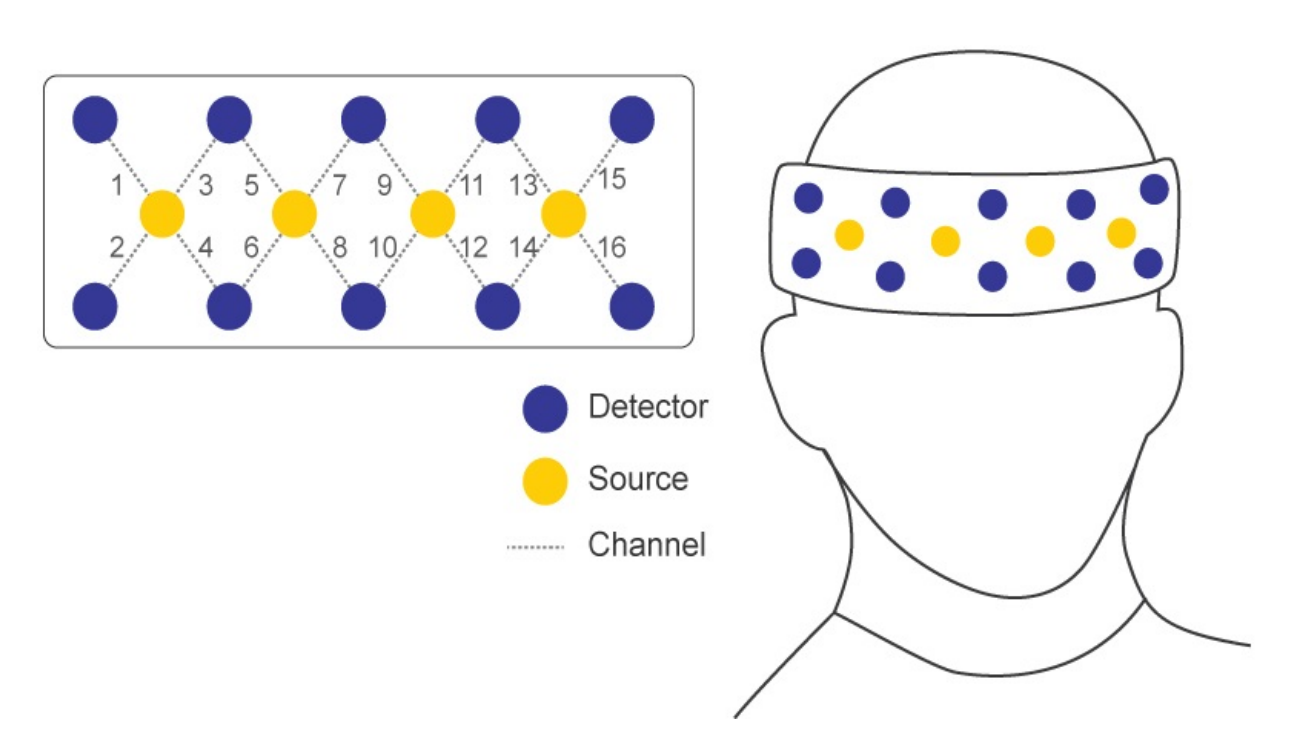
\includegraphics[width=0.7\linewidth]{../figures/source-detector-diagram}
%	\caption[fNIRS source-detector diagram]{The spatial arrangement of the source-detector pars placed on participants forehead.}
%	\label{fig:source-detector-diagram}
%\end{figure}


\subsection{NASA-TLX and Self assessment manikin scale (SAM)}
To assess operator perceived workload we used the paper version of the multidimensional subjective workload scale NASA-TLX \cite{nasatlx}.
The individual scales are presented in the following order: Mental demand, Physical demand, Temporal demand, Performance, Effort, and Frustration.
The NASA-TLX scores were obtained from participants after completing each web form conditions.

To capture participants emotional valence and arousal we used a 5 point self assessment mankin (SAM)\cite{bradley1994measuring}.  
The participants were asked to fill the questionnaire after each video watched. 
%First they state their emotional valence(negative or positive) by choosing between 1 and 5, where 5 is strongly perceived positive emotion, and 1 is considered strong negative emotion. Then, they fill the arousal level scale, where 1 indicates low perceived arousal or boredom, and 5 signifies high perceived arousal or high level of excitement. Each of the subscales is supported by image visualisations illustrating the affective state.

%\subsubsection{Sound recording}
%The participants voice was recorded during the experiment using researchers mobile phone. The data was used to transcribe the user comments.

\subsection{Procedure}

Three video clips of automotive accidents were selected, in order to simulate the conditions before the filling of insurance claim.
The video clips of the accidents were chosen to be lightweight avoiding any scenes of gore, injured bodies, or fatalities. 
All of the accidents happened in low speed.

\begin{figure}[h]
	\centering
	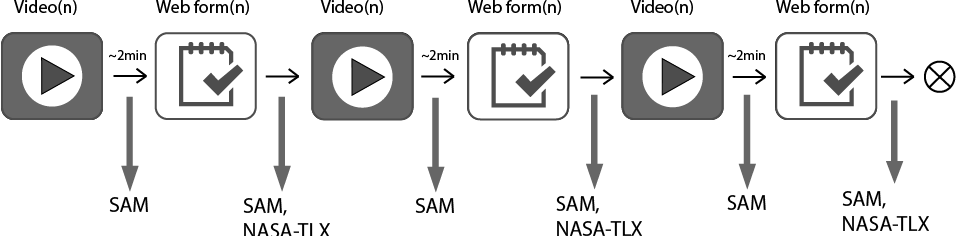
\includegraphics[width=\linewidth]{../figures/study-procedure}
	\caption[study procedure]{The image illustrates, the study procedure followed in this experiment.}
	\label{fig:study-procedure}
\end{figure}

Participants followed the procedure illustrated by Figure \ref{fig:study-procedure}. 
The three study conditions were counterbalanced using Latin square, to avoid learning effects.
%Also, because of ethical considerations that the participant should not enter personal data in the web form, a artificial personal credentials were provided, that she should fill in the web forms. 
Fourth, after the video capture and the fNIRS device were started, participants were asked to relax, in order to record a baseline of the hemodynamic activity while participants are at rest. Next, they are asked to open one of the three videos, depending on the counterbalancing order. 
They were instructed by the researcher to manually start certain condition or video. 
After watching of the video was finished, participants fill SAM subjective scale. 
Fifth, there was approximately 2 minute waiting period between the video and the web form filling task, so that participant's memory is not fresh. Finally, after participant completed the web form the NASA-TLX scales was given to be completed. 
This process was repeated three times, following the within subjects experimental design with counter balancing between the videos and the web forms.

\end{document} 